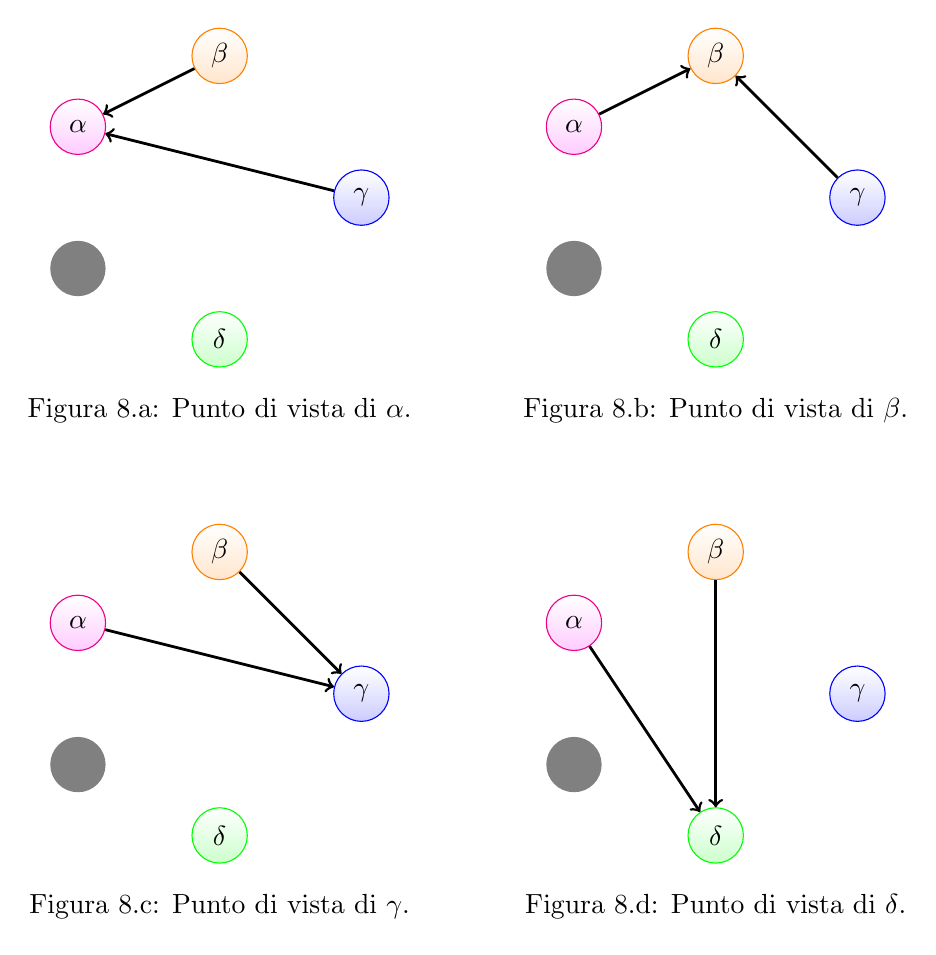
\begin{tikzpicture}[scale=.9]

\tikzset{mynode/.style={circle,minimum size=20pt,inner sep=0pt,draw, top color=white ,bottom color=blue!20, blue,text=black},}
\tikzset{mynode2/.style={circle,minimum size=20pt,inner sep=0pt,draw, top color=white ,bottom color=magenta!20, magenta,text=black},}
\tikzset{mynode3/.style={circle,minimum size=20pt,inner sep=0pt,draw, top color=white ,bottom color=orange!20, orange,text=black},}
\tikzset{mynode6/.style={circle,minimum size=20pt,inner sep=0pt,draw, top color=white ,bottom color=green!20, green,text=black},}
\tikzset{mynode7/.style={circle,fill=gray,minimum size=20pt,inner sep=0pt,},draw}
\tikzset{label/.style={minimum size=15pt,inner sep=0pt,},}


%ALPHA  
\draw (0,0) node [mynode7] () {};
\draw (0,2) node [mynode2] (alfa1) {$\alpha$};
\draw (4,1) node [mynode] (gamma1) {$\gamma$};
\draw (2,-1) node [mynode6] (delta1) {$\delta$};
\draw (2,3) node [mynode3] (beta1) {$\beta$};

\draw[->,line width=1pt] (beta1) -- (alfa1);
\draw[->,line width=1pt] (gamma1) -- (alfa1);
\draw(2,-2) node[label] (l) {Figura 8.a: Punto di vista di $\alpha$.};
  

%BETA  
\draw (7,0) node [mynode7] () {};
\draw (7,2) node [mynode2] (alfa2) {$\alpha$};
\draw (11,1) node [mynode] (gamma2) {$\gamma$};
\draw (9,-1) node [mynode6] (delta2) {$\delta$};
\draw (9,3) node [mynode3] (beta2) {$\beta$};

\draw[->,line width=1pt] (alfa2) -- (beta2);
\draw[->,line width=1pt] (gamma2) -- (beta2);
\draw(9,-2) node[label] (l) {Figura 8.b: Punto di vista di $\beta$.};
     
 
 

%GAMMA
\draw (0,-7) node [mynode7] () {};
\draw (0,-5) node [mynode2] (alfa3) {$\alpha$};
\draw (4,-6) node [mynode] (gamma3) {$\gamma$};
\draw (2,-8) node [mynode6] (delta3) {$\delta$};
\draw (2,-4) node [mynode3] (beta3) {$\beta$};

\draw[->,line width=1pt] (alfa3) -- (gamma3);
\draw[->,line width=1pt] (beta3) -- (gamma3);
\draw(2,-9) node[label] (l) {Figura 8.c: Punto di vista di $\gamma$.};
  


%DELTA
\draw (7,-7) node [mynode7] () {};
\draw (7,-5) node [mynode2] (alfa4) {$\alpha$};
\draw (11,-6) node [mynode] (gamma4) {$\gamma$};
\draw (9,-8) node [mynode6] (delta4) {$\delta$};
\draw (9,-4) node [mynode3] (beta4) {$\beta$};

\draw[->,line width=1pt] (alfa4) -- (delta4);
\draw[->,line width=1pt] (beta4) -- (delta4);
\draw(9,-9) node[label] (l) {Figura 8.d: Punto di vista di $\delta$.};
      
     
\end{tikzpicture}